\section{\name\ Architecture}
\label{arch}

Simplifying the design, planning, execution, and analysis of experiments, \name\
is comprised of four main parts as shown in Figure~\ref{lem-plan}.  A command
generator reads a simple experiment description and produces a command to run
each \sub.  The \subs\ are then passed to the\ \dispatcher\ who is responsible
for dispatching each.  As each \sub\ is executed, its output is parsed by
\Term{transducers} who insert parsed \kv\ pairs into a SQL server.  The user
then uses DBViz, which queries the SQL server, to visualize and analyze their
results.  Depending on this analysis, the user can modify their experiment
description and repeat the cycle.

\subsection{Command Generation}

\name\ provides a \cg\ engine which reads a description of the experiment,
computes all \subs\ needed to complete the experiment, and
produces a command to execute each \sub.  
For example, for an experiment wishing to study the
effect of a set of independent variables, the user merely specifies an array of
every target value for each independent variable.  If multiple independent
variables are specified, the \cg\ produces every possible combination of
commands.  The \cg\ assumes that each \sub\ will be executed with 
\Term{mpirun}, although this can be over-ridden.  The generated commands are 
then passed to the \dispatcher\ who initially just lists the commands so that 
the user can verify that the commands have been correctly generated; once 
verified, the \dispatcher\ can either submit the commands to the scheduling 
system or run them synchronously in the foreground. 

\begin{figure*}[tb]
\subfloat[Experiment Description]{\label{mdtest-desc}
\lstinputlisting{examples/mdtest.py}}
\hspace{20pt}
\subfloat[Generated Commands]{\label{mdtest-commands}
\lstinputlisting{examples/mdtest.out}}
\mycaption{mdtest}{Command Generation.}{
On the left is a simple experiment description for the parallel
metadata benchmark \Term{mdtest}.  Lists are specified 
the \Term{-l} and the \Term{-z} options whereas just a single value
is specified for the \Term{-d} and \Term{-b} options.  The options list for 
\Term{mpi}
specifies that each generated command should be run at different sizes 
(passed to \Term{mpirun} with the \Term{-np} option. 
This example also shows how transducers can be 
specified to the \cg.  The right side shows the commands generated
from this experiment description.  Note that the user can either create
an experiment description file as in the left column or can manually create
a list of commands like those on the right side.  The \cg\ will determine
whether it needs to automatically generate commands from a description file
or whether it merely reads the commands directly.  Once the \cg\ either
generates the commands or reads them in, it then passes them to the \dispatcher.
}
\end{figure*}


The simplest approach is to write a text file with one mpirun command in each
line; in this case, the \cg\ will pass each command directly to the
\dispatcher\ without modification.  For more complicated parameter studies,
\name\ provides a template where multiple list of parameters can be specified.
Figure~\ref{mdtest-desc} shows an example of an experiment description file for
the \Term{mdtest} parallel metadata benchmark.  This example shows how the
optional \Term{mpi\_options}, \Term{program\_options}, \Term{transducers}, and
\Term{transducer\_arguments} are used.  The command generator then creates all
possible commands from the permutations of the lists of options and arguments
as is shown in Figure~\ref{mdtest-commands}.  The \Term{--desc} argument is
parsed by the transducer, is removed from the arguments passed to
\Term{mdtest}, and is used as a tag for the experiment to easily group all of
the \subs\ for subsequent analysis.

Although the \cg\ can read from a simple list of mpirun commands, for any
reasonable parameter sweep, a description file is a drastic simplification.
Although this description file must be written in \Term{Python}, the basic
structure is already provided to the user in a template description file.  
So far two different users lacking any \Term{Python} experience have used
\name\ and were able to edit the provided template and start executing their
experiments within an hour. 

\subsection{\Dispatcher}

\name\ provides an \manager\ program \Term{run\_expr.py}.  To run an experiment,
the user executes the \manager\ by passing it either a description file or a
text list of commands.  After invoking the \cg\ to obtain a list of commands
from the file provided by the user, the \manager\ then passes these commands to
the \dispatcher.  The \manager\ program takes several command line options
which it passes to the \dispatcher such as the mode of dispatch, the number of
times to run each command, and whether to randomly shuffle the commands before
dispatching them.  The dispatch mode specifies how the \dispatcher\ should
dispatch each command; by default it merely lists the generated commands so
that the user can verify that the parameter study has been correctly configured
in the description file.  After verifying the list of commands, the user can
ask the \dispatcher\ (with command line options passed to the \manager) to run
the jobs synchronously in the foreground or to submit them to a scheduling
system.  

Additional command line options can be used to pass additional information to
the scheduling system.  Currently, \name\ only supports the \Term{moab}
scheduler although it can easily be modified to support other schedulers as
well; an earlier version of \name\ had support for both \Term{moab} and
\Term{PBS}.  

The \dispatcher\ also pulls default parameters from a configuration file which
is also written in Python.  This configuration file provides different
scheduling system parameters for different supercomputers.  For example, at
LANL we have populated our \name\ configuration file with information about the
number of cores on each node in our different supercomputers.  This information
is then passed to the scheduling system which needs to know how many nodes to
allocate for different numbers of requested processes (\eg\ to dispatch a 128
processor job on the LANL RRZ supercomputer, the \dispatcher\ reads the
configuration file to discover that RRZ has eight cores per node and therefore
requests sixteen nodes from the scheduling system).  We also include
information about the default filesystem for each supercomputer; although the
naming conventions on each supercomputer are mostly consistent, some
supercomputers do have different paths to their parallel storage systems.  By
specifying a default value for each supercomputer, we can use a single
experiment description file across multiple supercomputers without modifying it
specifically for each. 

Some of the functionality of the \dispatcher\ might seem redundant since users
can access scheduling systems directly; however, we believe that this
redundancy is actually one contribution of \name\ in that it abstracts the
scheduling system away.  Users create an experiment description file, and a
configuration file, and can then dispatch commands on any scheduling system on
any supercomputer without having to modify any of their scripts
since \name\ transparently interacts with the scheduling system for them.

\subsection{Transducers}

As command generation and dispatch assist the planning and execution phases of
an experiment \lifecycle, so do the \name\ \Term{transducers} assist in the
measurement phase.  The term transducers is borrowed from Semantic File Systems
(SFS)~\cite{gifford-sfs}.  Just as transducers in SFS create searchable
semantic information about files, transducers in \name\ create searchable
semantic information about each \sub.  \name\ provides a general transducer
which collects information about every \sub; this transducer can be augmented
by the user to collect information specific to the application.  As is shown in
Figure~\ref{mdtest-commands}, the transducer parses the output of each \sub,
records the command line of each, collects additional information about the
execution environment, and then inserts all of this collected information as
\kv\ pairs into a SQL server.  Some of the \kv\ pairs collected from each \sub\
are as follows:

\begin{quote}
\begin{itemize}
\mydefinition{application}{Name of the application}
\mydefinition{commandline}{Command line used}
\mydefinition{description}{Optional experiment tag}
\mydefinition{epoch}{UNIX epoch at time of execution}
\mydefinition{hostlist}{A list of each compute node}
\mydefinition{numhosts}{Number of compute nodes used}
\mydefinition{retval}{Return value}
\mydefinition{system}{Name of the supercomputer}
\mydefinition{username}{Username of the submitting user}
\mydefinition{walltime}{Total runtime}
\end{itemize}
\end{quote}

The provided transducer can be easily extended by users comfortable with
regular expressions who can parse the application output to gather additional
\kv\ pairs specific to their applications.  For example, our transducer for
\Term{mdtest} requires only 200 lines to parse the output and collect
semantic information about the configuration and results for each \sub. 

\subsection{\label{sec-analysis}Visualization and Analysis}

\begin{figure*}[tb]
\centering
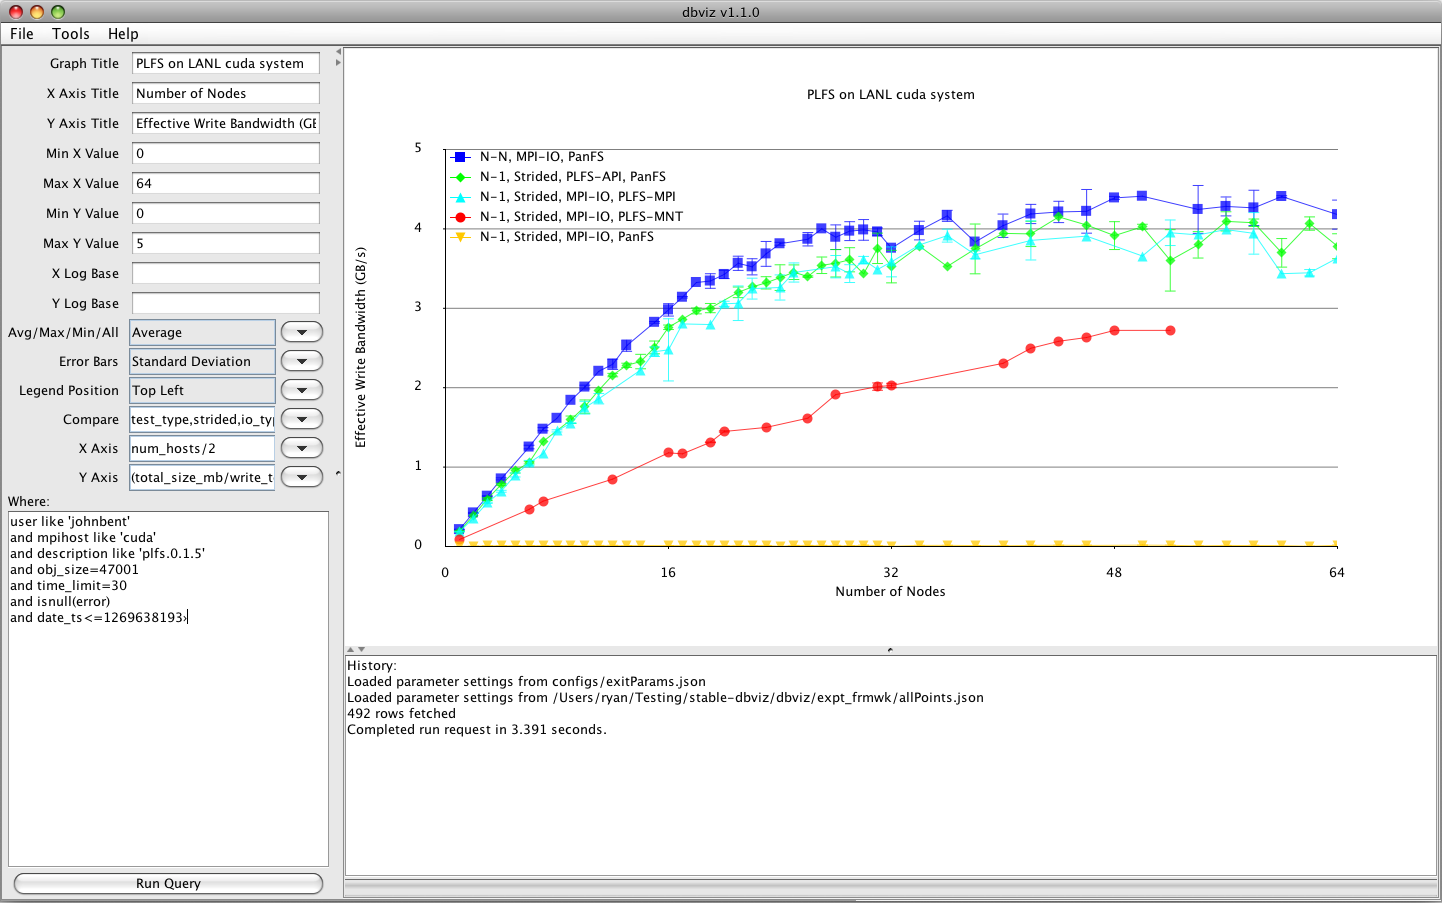
\includegraphics[width=0.7\textwidth]{dbvizGraphsAndConfigs/screenShot.png}
\mycaption{dbviz-screen}{Interactive Data Exploration.}{This screenshot of
\dbviz\ shows how a graph is generated from a specified filter, \xaxis,
\yaxis\, and a set of columns to compare.}
\end{figure*}

To enable interactive data exploration, we have developed \dbviz, a data
analysis tool written in \Term{Java Swing}.  This tool pulls data from any
\Term{SQL} database and plots it according to the user's specifications.  The
resulting graph is interactive which allows the user to more closely analyze
the data.  After ascertaining the table to be queried, \dbviz\ fetches the
schema and uses it to populate pull-down menus which are used to specify which
fields to display on the axes and which fields to use to create comparisons
(\ie\ different lines in the resulting graph).  This eliminates the need for
the user to remember the exact schema.  Although the user can use the pull-down
menus as a shortcut, the user can also request that more complicated operations
be performed.  For example, an axis can be just a single field or it can be a
function of multiple fields and constants; this could be used for instance to
create a bandwidth by dividing a size field by a time field.  When the user
does create more complicated functions for the axes or the compare fields,
these are remembered persistently by \dbviz\ and are added to the pull-down
menus so that they need be created only once.

\begin{figure*}[tb]
  \centering
  \subfloat[\label{nonrandom}Linespoints]{
    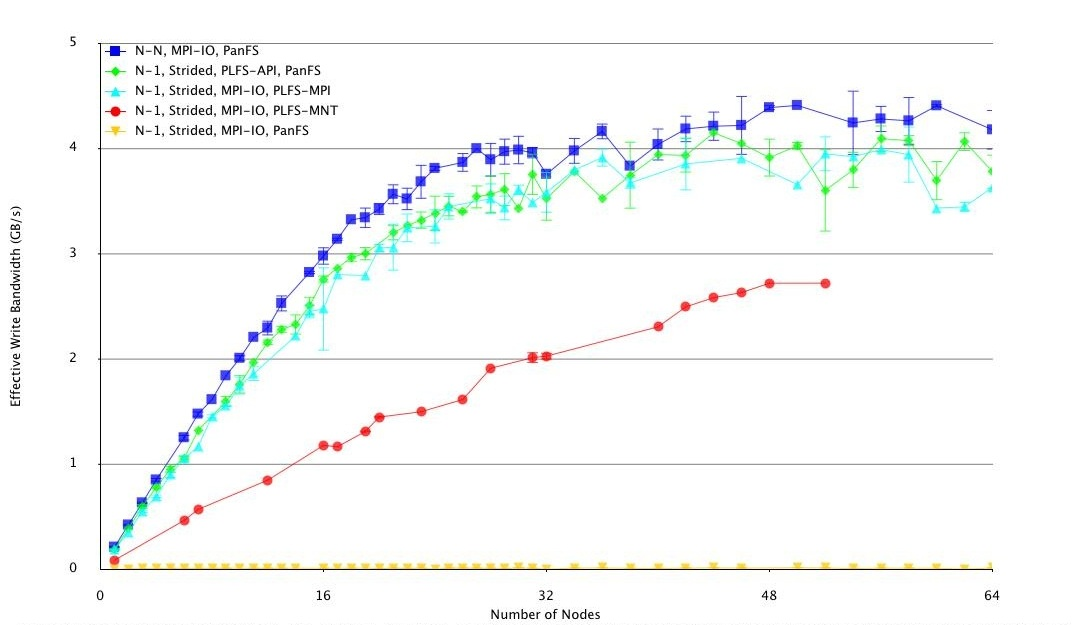
\includegraphics[width=0.3\textwidth,height=\figheight]{dbvizGraphsAndConfigs/allPoints.jpg}
  }
  \subfloat[\label{random}XY-scatter]{
    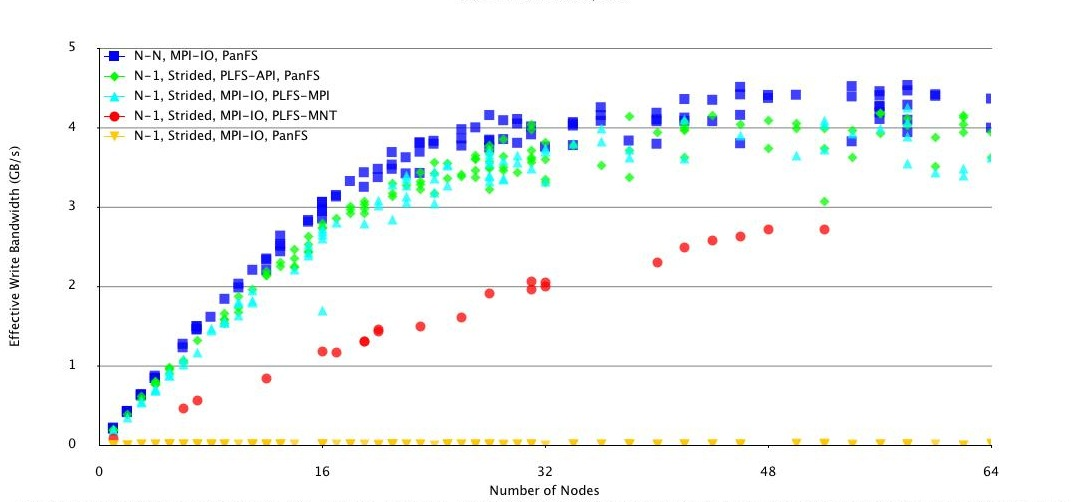
\includegraphics[width=0.3\textwidth,height=\figheight]{dbvizGraphsAndConfigs/allPointsAllScatter.jpg}
  }
  \subfloat[\label{random-full}Bars]{
    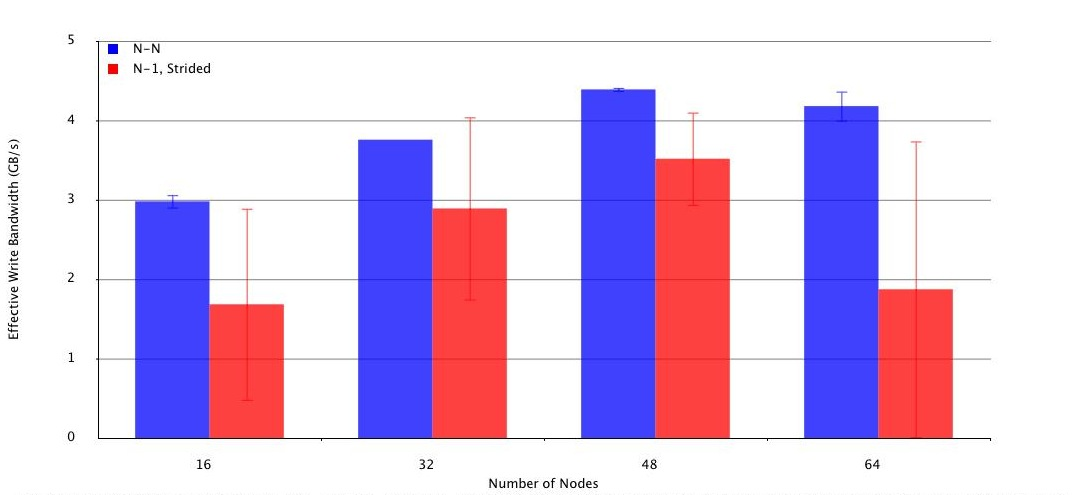
\includegraphics[width=0.3\textwidth,height=\figheight]{dbvizGraphsAndConfigs/allPointsBarGraph.jpg}
  }
  \mycaption{fig-dbviz}{Visualization Flexibility.}{
After \name\ populates a database with \kv\ pairs collected by transducers,
\dbviz\ allows interactive exploration of that data.  These figures 
show typical visualizations where a filter has been applied to the database,
and a visualization using the resulting rows is displayed.  One line (or bar) is
produced for each set of parameters that the user wishes to compare as a
function of specified values for both axes. The axes values can be a single
field or they can be arbitrarily complex combinations of multiple fields and
constants (\eg\ to show a bandwidth in GB/s, the user might specify that the
\yaxis\ should be a field dividing the number of bytes by a time and then 
dividing that again by a gigabyte).  The figure on the left shows an aggregation of
multiple points into mean values with standard deviations.  In the middle is
the same data in an xy-scatter plot; the scatter plot is useful because it allows
the user to easily identify outlying data.  The interactivity is vital here
as a user can click on an outlying data point and \dbviz\ will transparently
query the database and display a table of all \kv\ pairs for that outlier.
Finally, \dbviz\ can produce bar-graphs as well as in the figure on the right.
}
\end{figure*}



After specifying the columns that should be displayed on the \xaxis\ and the
\yaxis, a filter (\eg\ an \Term{SQL} \Term{WHERE} clause) can also be
specified.  The filter allows the user to be more selective about the data that
will be returned.  By specifying a set of columns to be compared, different
configurations can be compared.  Currently, the available formats of the plots
are linespoints, xy-scatter, and bar graphs as is illustrated in
Figure~\ref{fig-dbviz}.  \dbviz\ allows sessions to be saved so that 
interesting data explorations and interactive sessions can be interrupted
and resumed.  These saved sessions are stored in text files which allows them
to be easily shared between users. 

There are two important features in \dbviz\ that make its interactivity so
valuable.  One is \Term{outlier analysis}; the other is \Term{hidden difference
search}.  

\subsubsection{Outlier analysis}
Outlier analysis is available in xy-scatter plots; the user can click
on any point and \dbviz\ will transparently query the database and present
every \kv\ pair for that point thereby allowing the user to quickly discover
the particular data for any \sub; we have found this to be of particular value
for analyzing outliers.  

\subsubsection{Hidden difference search}
Hidden difference search is another feature provided
by \dbviz\ to help the user refine their analysis.  Hidden differences are
caused by incompatible data being accidentally combined when the user specifies
an imprecise filter or set of comparison fields.  When the user suspects that
the visualization lacks sufficient precision, hidden difference search can
quickly identify suspect keys which need to be segregated or filtered to
increase analytical precision.

Both outlier analysis and
hidden difference search will be further illustrated by means of example in
Section~\ref{eval}.

\subsection{Monitoring and Replay}

By inserting executed commands into a \Term{SQL} server, \name\ allows
interactive data exploration as discussed above in Section~\ref{sec-analysis}.
In addition, \name\ provides two additional programs that utilize the
\Term{SQL} server.  \Term{replay\_expr.py} takes a \Term{SQL} filter (\ie\ a
WHERE statement), queries the database for all previously executed commands
matching that filter, and passes them to the \dispatcher.  This is frequently
utilized at our site to check differences in platform performance following a
configuration change such as an upgrade to the operating system or changing the
buffer size on a network switch.  In such cases, the platform administrators
will conduct a measurement, giving it a unique tag, before making the change;
after the change, they merely use \Term{replay\_expr.py} to rerun that same
experiment.  Following the replay, they can use \dbviz\ to check for changes in
performance.  Although we use \name\ at our site primarily for platform
measurement and observation, it is applicable to any HPC experiment.  

A second tool that leverages the database is \Term{check\_expr.py} which takes
both a \Term{SQL} filter and an experiment description file.  By using the
command generator to generate the necessary \subs\ from the description file,
\Term{check\_expr.py} can then determine which have not yet been dispatched by
querying for each in the database.  The uncompleted \subs\ can then optionally
be passed to the \dispatcher\ to resubmit them.  Although this functionality
can also be achieved by querying the scheduling system, doing so within \name\
allows the user a single abstraction for interacting with multiple different
scheduling systems.  Additionally, we frequently encounter situations where the
scheduling systems' queues are purged by the administrators; in such cases,
querying the database is the simplest way to check progress of the experiment.
Finally, this approach drastically simplifies checking progress when the \subs\
have been spread across multiple computing sites, especially when each uses
different scheduling systems. 
